The database was designed in a way that reduces redundant information to a
minimum. The complete structure diagram is shown in Figure \ref{fig:dbstructure}
(page \pageref{fig:dbstructure}). All tables except the ``ests'', ``hmmsearch'',
and ``blast'' tables are used to store information about the amino acid or
nucleotide sequences that belong to either an ortholog set or a proteome of a
core taxon, or both. 

All tables have an ``id'' column with an auto-incremented integer as a unique
identifier. Normally, this identifier is used in \code{JOIN} queries that
reference other tables. The tables ``aaseqs'' and ``ntseqs'' contain the
amino acid or nucleotide sequences, respectively, that belong to the ortholog
sets. One of these tables is (or both are, if nucleotide sequences are present)
referenced to a sequence pair in the table ``sequence\_pairs''. The table
``set\_details'' contains a shorthand name for each ortholog set along with its
longer name or description. The ``id'' columns can be used to, \eg, construct a
SQL query that outputs all amino acid sequences that belong to a given ortholog
set (see \autoref{fig:db-orthoset} for this example). 

The tables ``aaseqs'' and ``ntseqs'' also contain amino acid and nucleotide
sequences that make up the reference proteomes and genomes, respectively. A
subset of these sequences is part of the ortholog sets. The proteome and genome
are commonly referred to and published as ``official gene set'' (OGS). Multiple
OGS versions of the same species can be stored concurrently; they are
distinguished by their version number in the database. Both OGS and EST data
can be of either nucleotide or amino acid sequences; the sequence type column is
referenced to the table ``types'', which has only two records---``nt'' for
nucleotide and ``aa'' for amino acid sequences---and serves only as a labeling
table.

All tables that contain sequence data, \ie, ``aaseqs'', ``ntseqs'', and
``ests'' have a column that holds a user ID. The table ``users'' can be
referenced to identify a username. This was introduced to connect the uploading
of a amino acid or nucleotide sequence dataset to a specific user in order to
facilitate separation of multiple datasets by different researchers in the same
database.



\begin{figure}[h]
	\centering
	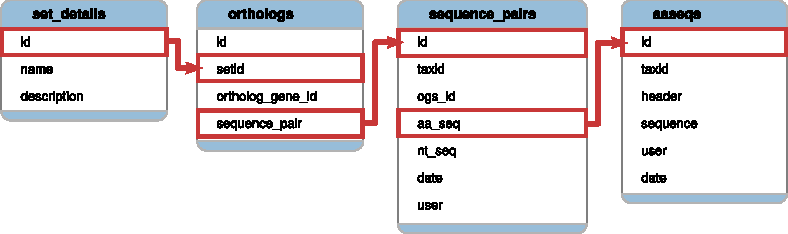
\includegraphics{img/db-orthoset.pdf}
	\caption[Database table connections for a given ortholog set]{
		\pname database structure for a given ortholog set. Each rounded rectangle
		represents a table with named columns. The red path delineates the
		\code{JOIN} query structure that returns all amino acid sequences (stored in
		the table ``aaseqs'') that belong to a given ortholog set. Ortholog set
		information is stored in the table ``set\_details''.
	}
	\label{fig:db-orthoset}
\end{figure}


\begin{figure}[ht]
	\centering
	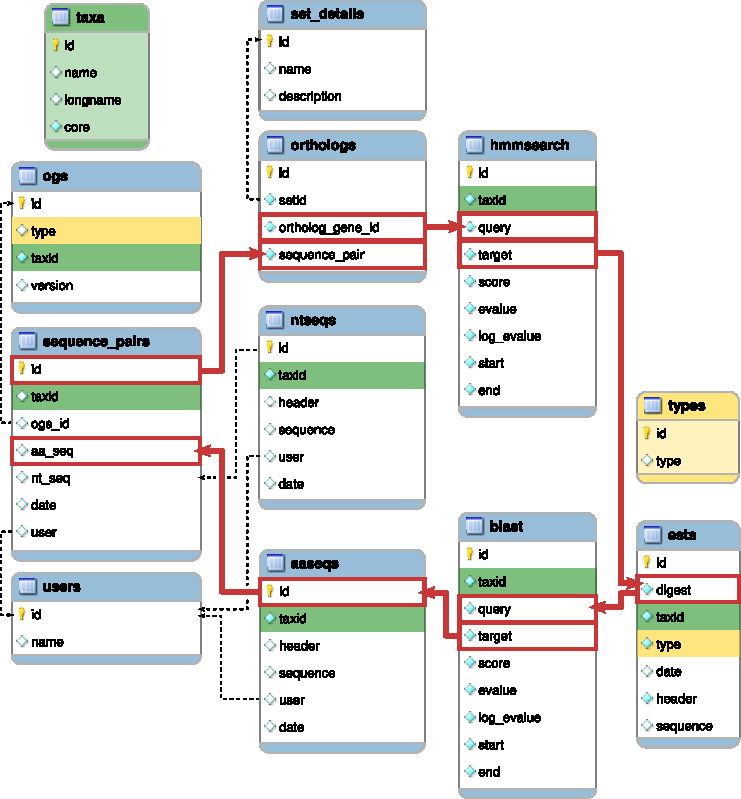
\includegraphics[width=\textwidth]{img/dbstructure.pdf}
	\caption[\pname database structure]{
		\pname database structure. Each rectangle represents a table with named
		columns. Note the circular path (red) that can be drawn across the tables and
		that is used in \code{JOIN} queries in order to construct a graph of
		orthologous relationships. Green table columns are referenced to the ``taxa''
		table, and yellow table columns are referenced to the ``types'' table. Dotted
		lines are secondary references.
	}
	\label{fig:dbstructure}
\end{figure}




